\documentclass[border=10px]{standalone}
\usepackage{tikz}
\usepackage[]{circuitikz}

\begin{document}
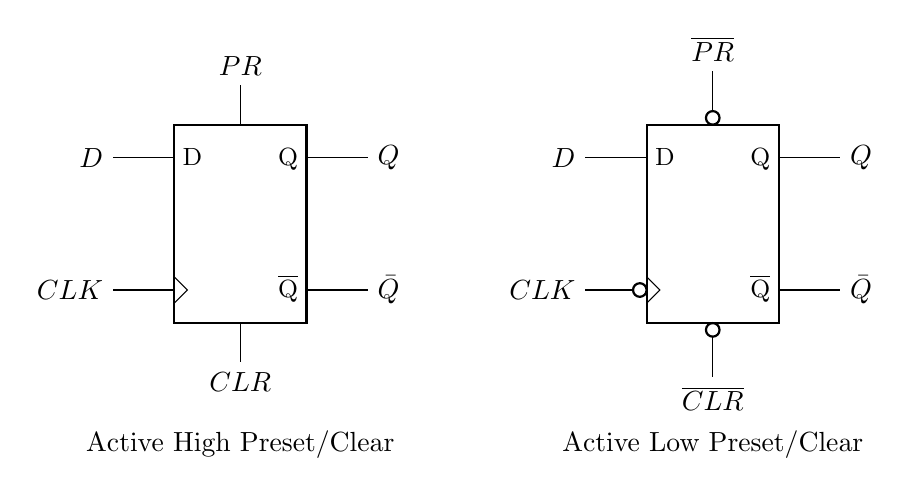
\begin{tikzpicture}
    \ctikzset{logic ports=ieee}
    % Left: Positive Edge D-FF with Async Positive Preset/Clear
    \node [flipflop D] (FF1) at (0,0) {};
    \draw (FF1.pin 1) -- ++(-0.5,0) node[left] {$D$};
    \draw (FF1.pin 3) -- ++(-0.5,0) node[left] {$CLK$};
    \draw (FF1.pin 6) -- ++(0.5,0) node[right] {$Q$};
    \draw (FF1.pin 4) -- ++(0.5,0) node[right] {$\bar{Q}$};
    
    % Positive Logic: No bubbles
    \draw (FF1.bup) -- ++(0,0.5) node[above] {$PR$};
    \draw (FF1.bdown) -- ++(0,-0.5) node[below] {$CLR$};
    
    \node [below=2.5cm, align=center] at (FF1) {Active High Preset/Clear};

    % Right: Negative Edge D-FF with Async Negative Preset/Clear
    \node [flipflop D, flipflop def={n3=1, nd=1, nu=1}] (FF2) at (6,0) {};
    \draw (FF2.pin 1) -- ++(-0.5,0) node[left] {$D$};
    % Manual bubble for negative edge clock
   % \draw [fill=white] (FF2.pin 3) ++(-2pt,0) circle(2pt);
    \draw (FF2.pin 3) -- ++(-0.5,0) node[left] {$CLK$};
    
    \draw (FF2.pin 6) -- ++(0.5,0) node[right] {$Q$};
    \draw (FF2.pin 4) -- ++(0.5,0) node[right] {$\bar{Q}$};
    
    % Bubbles for Active Low
   % \draw [fill=white] (FF2.up) circle(2pt);
   % \draw [fill=white] (FF2.down) circle(2pt);
    
    % Offset lines to not overlap bubble
    \draw (FF2.up) -- ++(0,0.4) node[above] {$\overline{PR}$};
    \draw (FF2.down) -- ++(0,-0.4) node[below] {$\overline{CLR}$};

    \node [below=2.5cm, align=center] at (FF2) {Active Low Preset/Clear};

\end{tikzpicture}
\end{document}
